%% source: 2022-fa-redemption_midterm_01
%% tags: [asymptotic notation]
\begin{prob}

    Let $f(n) = n \cdot (\sin{n} + 1 )$. A plot of this function is shown below.

    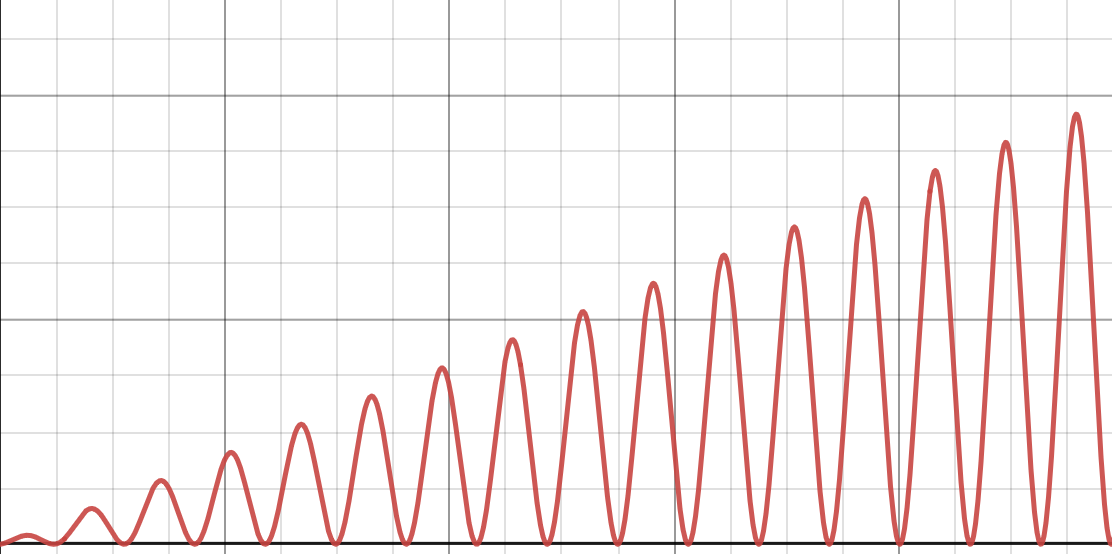
\includegraphics{./plot.png}

    True or False: $f(n) = \Theta(n)$.

    \tF{}

    \begin{soln}
        False.

        Remember that for $f(n)$ to be $\Theta(n)$, it has to be both upper- and lower-bounded
        by some \textit{positive} constant times $n$.
        This function is upper bounded by $O(n)$, but it doesn't have a lower bound
        of $\Omega(n)$. Therefore, it can't be $\Theta(n)$.

        In other words, there is no positive constant $c$ and no positive
        number $N$ such that $f(n) > c n$ for all $n > N$.

        If you had to describe this function in asymptotic notation, you could
        say that $f(n) = O(n)$ (and that would be a tight upper bound), but there
        is no lower bound, since the function keeps coming back down to zero.
    \end{soln}

\end{prob}
